% !TeX program = xelatex
\documentclass[UTF8,a4paper,12pt]{ctexart}

\usepackage[left=2.5cm,right=2.5cm,top=2.5cm,bottom=2.5cm]{geometry}
\usepackage{amsmath,amssymb,bm}
\usepackage{graphicx}
\usepackage{float}
\usepackage{booktabs}
\usepackage{array}
\usepackage{longtable}
\usepackage{multirow}
\usepackage{caption}
\usepackage{subcaption}
\usepackage{siunitx}
\usepackage{xcolor}
\usepackage{hyperref}
\usepackage{enumitem}
\usepackage{listings}

\hypersetup{
  colorlinks=true,
  linkcolor=black,
  citecolor=black,
  urlcolor=blue
}

\captionsetup{font=small,labelsep=space}
\setlist[itemize]{leftmargin=2em}
\setlist[enumerate]{leftmargin=2em}

\lstdefinestyle{matlabstyle}{
  language=Matlab,
  basicstyle=\ttfamily\small,
  keywordstyle=\color{blue!70!black},
  commentstyle=\color{green!40!black},
  stringstyle=\color{orange!70!black},
  numbers=left,
  numberstyle=\tiny\color{gray},
  stepnumber=1,
  numbersep=8pt,
  showstringspaces=false,
  breaklines=true,
  frame=single,
  rulecolor=\color{black!30},
  columns=flexible
}

\title{PUMA560 机械臂轨迹规划与运动学仿真实验报告}
\author{课程：智能机器人技术 \qquad 实验对象：PUMA560}
\date{\today}

\begin{document}

\maketitle

\begin{abstract}
本实验基于 MATLAB Robotics Toolbox，对经典六自由度工业机器人 PUMA560 开展运动学仿真分析。实验内容分为两个部分：其一是在笛卡尔空间中对末端执行器进行轨迹规划，并通过逆运动学求解和正运动学回代验证规划轨迹的可实现性与精度；其二是在关节空间中对关节变量进行平滑插值，并进一步分析由正运动学得到的末端轨迹以及由逆运动学恢复关节变量时出现的多解现象。实验结果表明，笛卡尔空间规划轨迹经过逆解和正解验证后，末端位置最大误差约为 $3.15\times 10^{-16}\,\si{m}$，处于数值计算精度范围内；关节空间规划中，关节角、角速度和角加速度曲线连续平滑，而由末端位姿反求得到的关节解与原始轨迹之间存在显著差异，说明逆运动学满足位姿等价但不一定保持关节解唯一。实验验证了 PUMA560 末端空间运动与关节空间运动之间的映射关系，加深了对正、逆运动学及轨迹规划方法的理解。
\end{abstract}

\noindent\textbf{关键词：}PUMA560；Robotics Toolbox；正运动学；逆运动学；笛卡尔空间轨迹规划；关节空间轨迹规划

\section{实验目的}

\begin{enumerate}
  \item 熟悉 MATLAB Robotics Toolbox 中 PUMA560 模型的调用方法与基本功能。
  \item 掌握串联机械臂正运动学与逆运动学的基本思想及其在仿真中的实现过程。
  \item 理解笛卡尔空间轨迹规划与关节空间轨迹规划的区别、联系及适用场景。
  \item 通过仿真结果分析末端位姿与关节变量之间的映射关系，并验证模型求解结果的正确性。
  \item 为后续开展机械臂动力学分析、控制算法设计与复杂路径规划实验奠定基础。
\end{enumerate}

\section{实验内容与任务}

本实验以 PUMA560 六自由度工业机器人为研究对象，围绕“轨迹规划与运动学验证”开展两项仿真分析：
\begin{enumerate}
  \item 在笛卡尔坐标系中进行末端执行器轨迹规划，并对轨迹点进行逆运动学求解，再通过正运动学回代验证轨迹执行结果。
  \item 在关节坐标系中进行关节轨迹规划，并由正运动学求得末端轨迹，再利用逆运动学恢复关节变量，分析逆解结果与原始关节轨迹的关系。
\end{enumerate}

实验中选取 Robotics Toolbox 内置姿态 $q_z$ 作为起始关节角，选取典型姿态 $q_r$ 作为目标关节角，具体为
\begin{equation}
q_z=[0,0,0,0,0,0],
\end{equation}
\begin{equation}
q_r=[0,\frac{\pi}{2},-\frac{\pi}{2},0,0,0].
\end{equation}
采样点数设为 $n=50$。

\section{实验原理与公式推导}

\subsection{PUMA560 机械臂模型}

PUMA560 为典型的六自由度串联关节型机械臂，前三个关节主要决定末端位置，后三个关节主要决定末端姿态。实验中调用 Robotics Toolbox 提供的 \texttt{mdl\_puma560} 建立其标准模型。根据工具箱内模型参数，可得到如表~\ref{tab:dh} 所示的 DH 参数。

\begin{table}[H]
  \centering
  \caption{PUMA560 模型的 DH 参数}
  \label{tab:dh}
  \begin{tabular}{cccccc}
    \toprule
    连杆 $i$ & 关节变量 $\theta_i$ & $d_i$/m & $a_i$/m & $\alpha_i$/rad & 关节类型 \\
    \midrule
    1 & $\theta_1$ & 0       & 0      & $\frac{\pi}{2}$  & 转动关节 \\
    2 & $\theta_2$ & 0       & 0.4318 & 0                & 转动关节 \\
    3 & $\theta_3$ & 0.15005 & 0.0203 & $-\frac{\pi}{2}$ & 转动关节 \\
    4 & $\theta_4$ & 0.4318  & 0      & $\frac{\pi}{2}$  & 转动关节 \\
    5 & $\theta_5$ & 0       & 0      & $-\frac{\pi}{2}$ & 转动关节 \\
    6 & $\theta_6$ & 0       & 0      & 0                & 转动关节 \\
    \bottomrule
  \end{tabular}
\end{table}

\subsection{正运动学}

采用 DH 法建模时，第 $i$ 个连杆从坐标系 $\{i-1\}$ 到坐标系 $\{i\}$ 的齐次变换矩阵为
\begin{equation}
{}^{i-1}\mathbf{T}_i=
\begin{bmatrix}
\cos\theta_i & -\sin\theta_i\cos\alpha_i & \sin\theta_i\sin\alpha_i & a_i\cos\theta_i \\
\sin\theta_i & \cos\theta_i\cos\alpha_i  & -\cos\theta_i\sin\alpha_i & a_i\sin\theta_i \\
0            & \sin\alpha_i              & \cos\alpha_i              & d_i \\
0            & 0                         & 0                         & 1
\end{bmatrix}.
\label{eq:Ai}
\end{equation}

因此，机械臂从基座到末端执行器的总变换矩阵为
\begin{equation}
{}^{0}\mathbf{T}_6={}^{0}\mathbf{T}_1 {}^{1}\mathbf{T}_2 {}^{2}\mathbf{T}_3 {}^{3}\mathbf{T}_4 {}^{4}\mathbf{T}_5 {}^{5}\mathbf{T}_6
=\prod_{i=1}^{6} {}^{i-1}\mathbf{T}_i.
\label{eq:fk}
\end{equation}

矩阵 ${}^{0}\mathbf{T}_6$ 的前三行第四列给出末端位置
\begin{equation}
\mathbf{p}=[x,y,z]^\mathrm{T},
\end{equation}
前三行前三列给出末端姿态旋转矩阵。实验中调用 \texttt{p560.fkine(q)} 实现式~\eqref{eq:fk} 的数值求解。

\subsection{逆运动学}

逆运动学的目标是在给定末端位姿 ${}^{0}\mathbf{T}_6$ 的条件下，求取相应关节变量向量 $\mathbf{q}$，其中
\begin{equation}
\mathbf{q}=[q_1,q_2,\ldots,q_6].
\end{equation}
由于 PUMA560 具有球腕结构，Robotics Toolbox 中的 \texttt{ikine6s} 可利用解析方法求解六自由度球腕机械臂的逆运动学。其本质是将问题分解为两部分：
\begin{enumerate}
  \item 根据末端位置求解前三个关节变量，使腕中心到达目标位置；
  \item 根据目标姿态与前三关节结果求解后三个关节变量，使末端姿态满足要求。
\end{enumerate}

由于三角函数的周期性与机构构型对称性，同一末端位姿通常对应多组关节解，因此逆运动学解一般不唯一。实验二中出现的关节恢复误差正是这一特性的具体体现。

\subsection{笛卡尔空间轨迹规划原理}

实验一先由起始关节角和目标关节角分别计算末端位姿
\begin{equation}
\mathbf{T}_{\text{start}}=\mathrm{FK}(q_z), \qquad
\mathbf{T}_{\text{end}}=\mathrm{FK}(q_r).
\end{equation}

随后采用 \texttt{ctraj} 在位姿空间中插值得到 $n$ 个连续轨迹点
\begin{equation}
\mathbf{T}_k=\mathrm{ctraj}\left(\mathbf{T}_{\text{start}},\mathbf{T}_{\text{end}},n\right), \qquad k=1,2,\ldots,n.
\label{eq:ctraj}
\end{equation}

对每个位姿点求解逆运动学，可得关节轨迹
\begin{equation}
\mathbf{q}_k=\mathrm{IK}(\mathbf{T}_k).
\end{equation}

再对 $\mathbf{q}_k$ 进行正运动学计算，得到回代验证位姿
\begin{equation}
\hat{\mathbf{T}}_k=\mathrm{FK}(\mathbf{q}_k).
\end{equation}

若仅比较位置精度，则验证误差可定义为
\begin{equation}
e_k=\left\|\mathbf{p}_k-\hat{\mathbf{p}}_k\right\|_2.
\label{eq:poserr}
\end{equation}

\subsection{关节空间轨迹规划原理}

实验二采用 \texttt{jtraj} 在关节空间中生成平滑轨迹。其本质为满足初末速度和加速度为零的五次多项式插值。令归一化时间变量为 $\tau=t/t_f$，则单关节轨迹可写为
\begin{equation}
q(\tau)=q_0+\left(10\tau^3-15\tau^4+6\tau^5\right)(q_f-q_0),
\label{eq:jtraj}
\end{equation}
对应角速度与角加速度分别为
\begin{equation}
\dot{q}(\tau)=\frac{1}{t_f}\left(30\tau^2-60\tau^3+30\tau^4\right)(q_f-q_0),
\end{equation}
\begin{equation}
\ddot{q}(\tau)=\frac{1}{t_f^2}\left(60\tau-180\tau^2+120\tau^3\right)(q_f-q_0).
\end{equation}

将规划得到的关节轨迹 $\mathbf{q}_k$ 代入正运动学，即可获得末端轨迹
\begin{equation}
\mathbf{T}_k=\mathrm{FK}(\mathbf{q}_k).
\end{equation}

再对每个末端位姿进行逆运动学恢复，得到
\begin{equation}
\mathbf{q}^{\mathrm{ik}}_k=\mathrm{IK}(\mathbf{T}_k).
\end{equation}

考虑到关节角具有 $2\pi$ 周期性，实验中采用
\begin{equation}
\mathbf{e}^{(q)}_k=\mathrm{atan2}\big(\sin(\mathbf{q}_k-\mathbf{q}^{\mathrm{ik}}_k),\,\cos(\mathbf{q}_k-\mathbf{q}^{\mathrm{ik}}_k)\big)
\label{eq:joint_err}
\end{equation}
对角度差进行归一化，从而得到关节恢复误差。

\section{实验步骤}

\subsection{实验一：笛卡尔空间轨迹规划与正运动学验证}

\begin{enumerate}
  \item 调用 \texttt{mdl\_puma560} 建立 PUMA560 机械臂模型，并设置初始关节角 $q_z$ 与目标关节角 $q_r$。
  \item 利用 \texttt{fkine} 求取起始位姿 $\mathbf{T}_{\text{start}}$ 与目标位姿 $\mathbf{T}_{\text{end}}$。
  \item 使用 \texttt{ctraj} 在笛卡尔空间生成 50 个末端插值位姿点。
  \item 对每个位姿点采用 \texttt{ikine6s} 求解关节变量，构成关节轨迹序列。
  \item 将求得的关节轨迹重新代入 \texttt{fkine}，得到末端执行器的回代轨迹，并计算位置误差。
  \item 绘制机械臂姿态图、轨迹对比图、位置分量曲线和误差曲线，对规划结果进行分析。
\end{enumerate}

\subsection{实验二：关节空间轨迹规划与逆运动学分析}

\begin{enumerate}
  \item 在相同起始与目标关节角条件下，调用 \texttt{jtraj} 生成 50 个采样点的关节轨迹 $\mathbf{q}$、角速度 $\dot{\mathbf{q}}$ 与角加速度 $\ddot{\mathbf{q}}$。
  \item 利用 \texttt{fkine} 计算每个采样点对应的末端位姿和末端空间轨迹。
  \item 对各时刻末端位姿再次使用 \texttt{ikine6s} 进行逆运动学求解，得到恢复关节角。
  \item 按式~\eqref{eq:joint_err} 计算原始关节轨迹与逆解恢复轨迹之间的角度误差。
  \item 绘制末端轨迹、关节角曲线、关节速度曲线、关节加速度曲线及逆运动学恢复误差曲线，并分析逆解多解性对结果的影响。
\end{enumerate}

\section{实验结果与分析}

\subsection{初始与目标姿态分析}

由正运动学计算可知，起始末端位置约为 $(0.4521,-0.15005,0.4318)\,\si{m}$，目标末端位置约为 $(0.0203,-0.15005,0.8636)\,\si{m}$。也就是说，实验过程中末端主要表现为 $x$ 方向减小、$z$ 方向增大，而 $y$ 方向基本保持不变。

\begin{figure}[H]
  \centering
  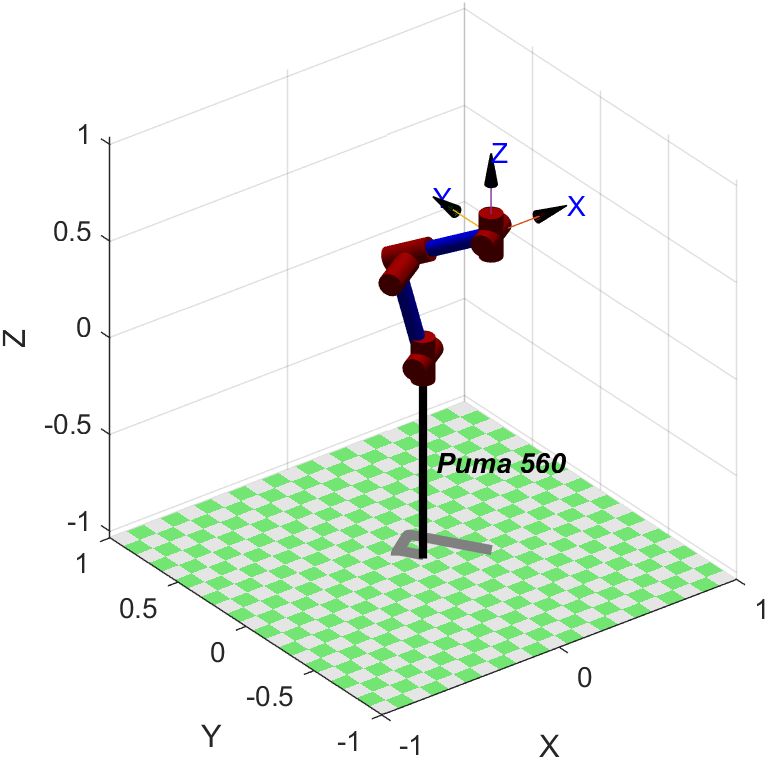
\includegraphics[width=0.55\textwidth]{figures/fig_mech_start.png}
  \caption{PUMA560 起始姿态（$q_z$）}
  \label{fig:mech_start}
\end{figure}

图~\ref{fig:mech_start} 给出了 PUMA560 在初始关节角 $q_z$ 下的空间姿态。此时机械臂处于较为展开的基础姿态，末端位于机械臂前上方，适合作为轨迹规划的起始状态。

\begin{figure}[H]
  \centering
  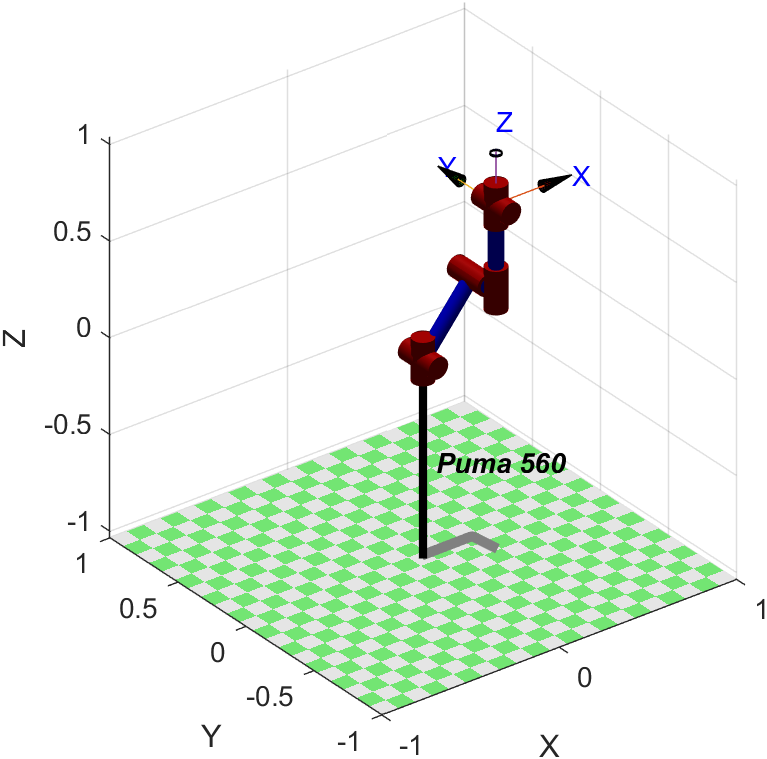
\includegraphics[width=0.55\textwidth]{figures/fig_mech_goal.png}
  \caption{PUMA560 目标姿态（$q_r$）}
  \label{fig:mech_goal}
\end{figure}

图~\ref{fig:mech_goal} 为目标关节角 $q_r$ 对应的机械臂姿态。与初始姿态相比，第二、第三关节发生了明显变化，使机械臂整体向上抬起，末端高度增加。这一姿态变化与后续轨迹图中 $z$ 坐标上升的趋势一致。

\subsection{实验一结果：笛卡尔空间轨迹规划与正运动学验证}

\begin{figure}[H]
  \centering
  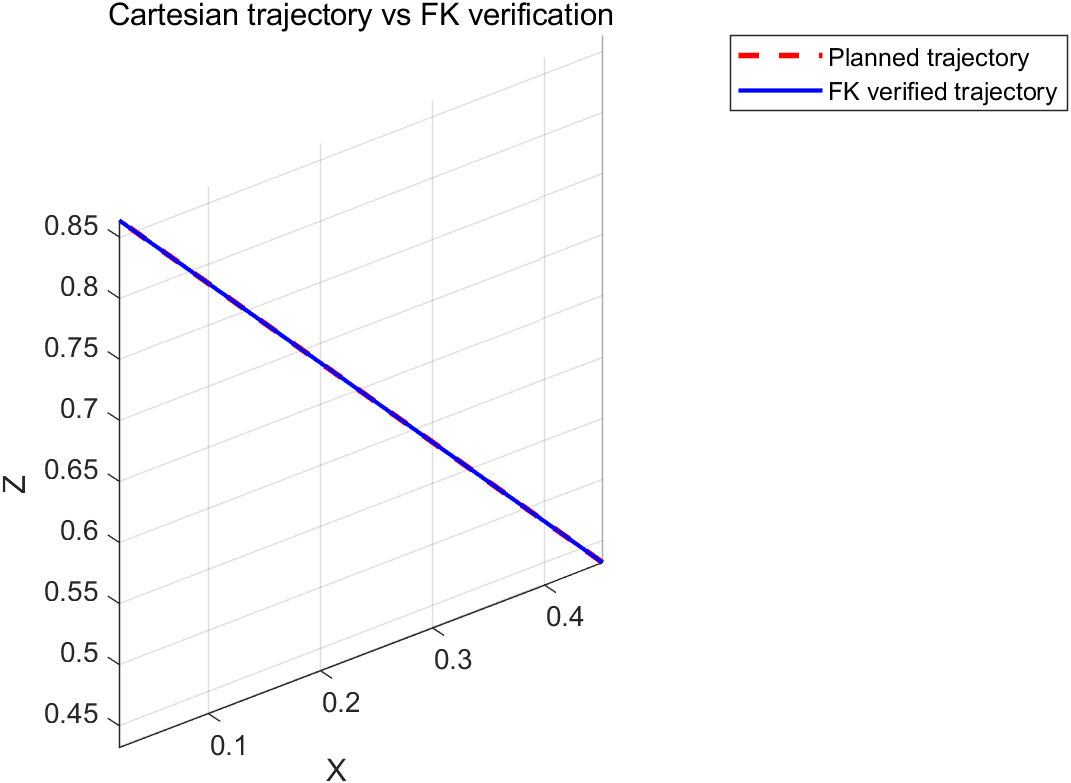
\includegraphics[width=0.70\textwidth]{figures/fig_exp1_traj_compare.png}
  \caption{笛卡尔空间规划轨迹与正运动学验证轨迹对比}
  \label{fig:exp1_traj_compare}
\end{figure}

图~\ref{fig:exp1_traj_compare} 中虚线表示在笛卡尔空间中直接规划得到的目标轨迹，实线表示对各轨迹点进行逆运动学求解后，再通过正运动学回算得到的验证轨迹。两条曲线几乎完全重合，说明逆运动学求得的关节变量能够准确实现所规划的末端位姿，且正运动学回代结果与原始规划一致。

\begin{figure}[H]
  \centering
  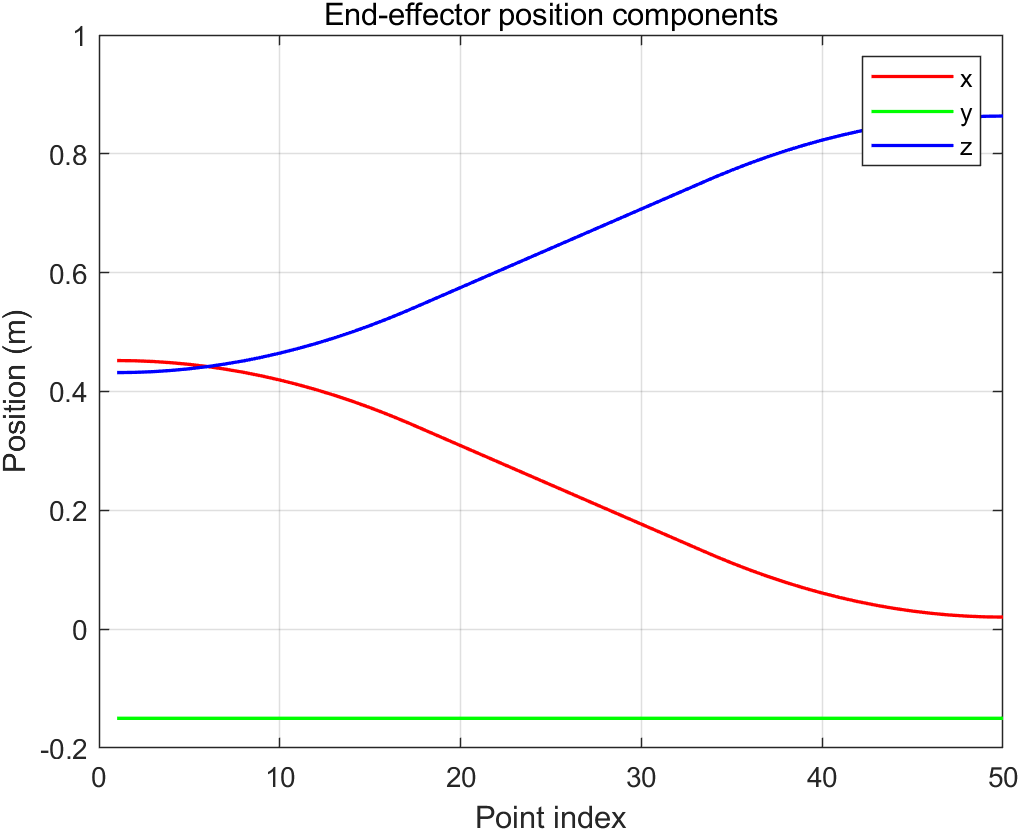
\includegraphics[width=0.78\textwidth]{figures/fig_exp1_xyz_components.png}
  \caption{实验一中末端位置三个分量的变化曲线}
  \label{fig:exp1_xyz_components}
\end{figure}

图~\ref{fig:exp1_xyz_components} 反映了实验一规划轨迹中末端位置分量随采样点的变化规律。可以看出：
\begin{itemize}
  \item $x$ 分量由约 \SI{0.4521}{m} 逐步减小至约 \SI{0.0203}{m}；
  \item $y$ 分量基本保持在 \SI{-0.15005}{m} 附近，变化极小；
  \item $z$ 分量由约 \SI{0.4318}{m} 平滑增大至约 \SI{0.8636}{m}。
\end{itemize}
这说明笛卡尔空间轨迹规划的主导运动是“前伸量减小、末端抬升”，轨迹整体呈现平滑过渡。

\begin{figure}[H]
  \centering
  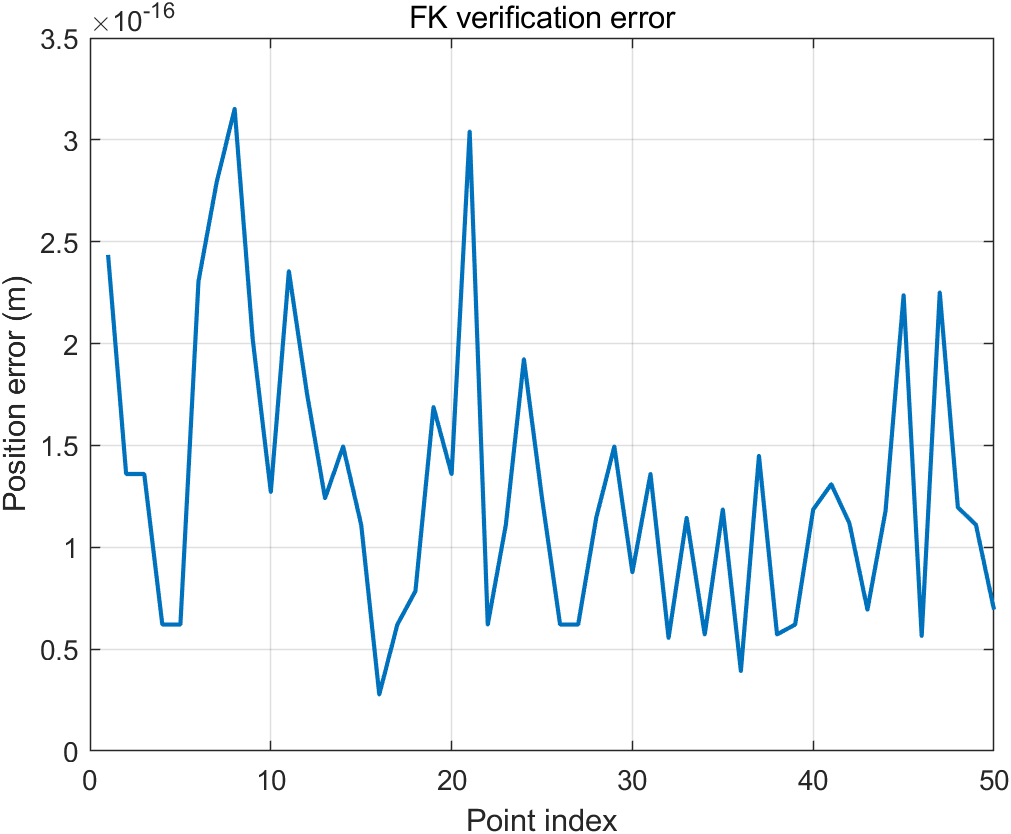
\includegraphics[width=0.78\textwidth]{figures/fig_exp1_fk_error.png}
  \caption{实验一中正运动学验证的位置误差曲线}
  \label{fig:exp1_fk_error}
\end{figure}

图~\ref{fig:exp1_fk_error} 为笛卡尔轨迹规划结果经逆解和正解验证后的位置误差曲线。误差虽有轻微起伏，但数量级极小，其最大值为
\begin{equation}
e_{\max}=3.1524\times 10^{-16}\ \si{m},
\end{equation}
平均值约为 $1.2942\times 10^{-16}\,\si{m}$。这一结果表明，误差基本来源于浮点运算舍入，而非算法本身的规划偏差，因此可认为实验一中的轨迹规划与正运动学验证结果是完全一致的。

综上，实验一验证了以下结论：在末端位姿轨迹可达的条件下，PUMA560 机械臂能够通过逆运动学实现笛卡尔空间中给定的轨迹要求，且回代得到的执行轨迹与原始规划轨迹高度一致，证明模型与求解流程正确。

\subsection{实验二结果：关节空间轨迹规划与逆运动学分析}

\begin{figure}[H]
  \centering
  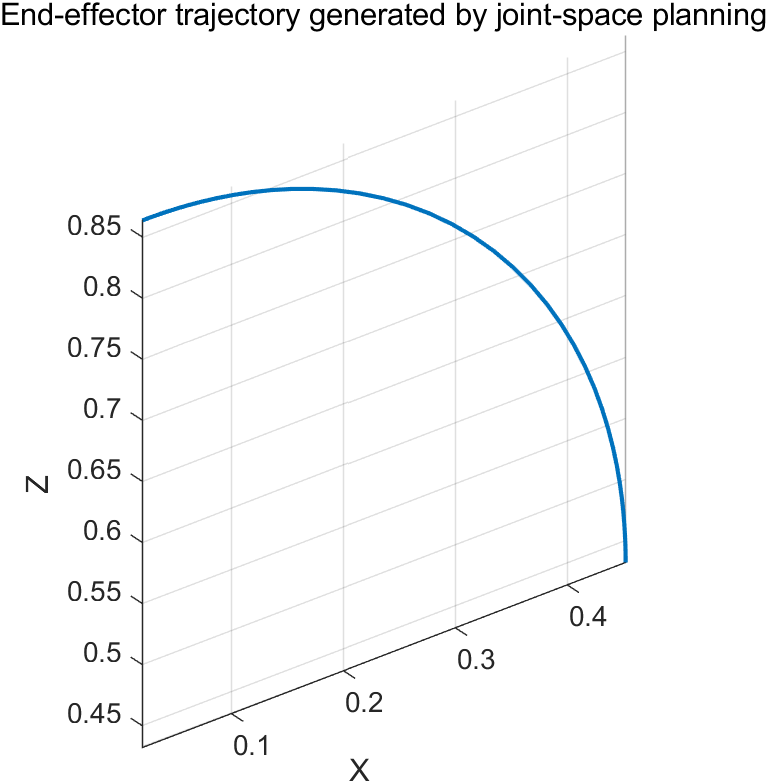
\includegraphics[width=0.70\textwidth]{figures/fig_exp2_ee_traj.png}
  \caption{关节空间规划对应的末端执行器空间轨迹}
  \label{fig:exp2_ee_traj}
\end{figure}

图~\ref{fig:exp2_ee_traj} 给出了由关节空间轨迹经正运动学映射得到的末端空间轨迹。与实验一中直接在笛卡尔空间得到的近似直线型轨迹不同，这里末端路径呈现明显的弯曲形态，说明关节空间插值并不保证末端在空间中的运动轨迹为直线，只能保证关节变量随时间平滑变化。

\begin{figure}[H]
  \centering
  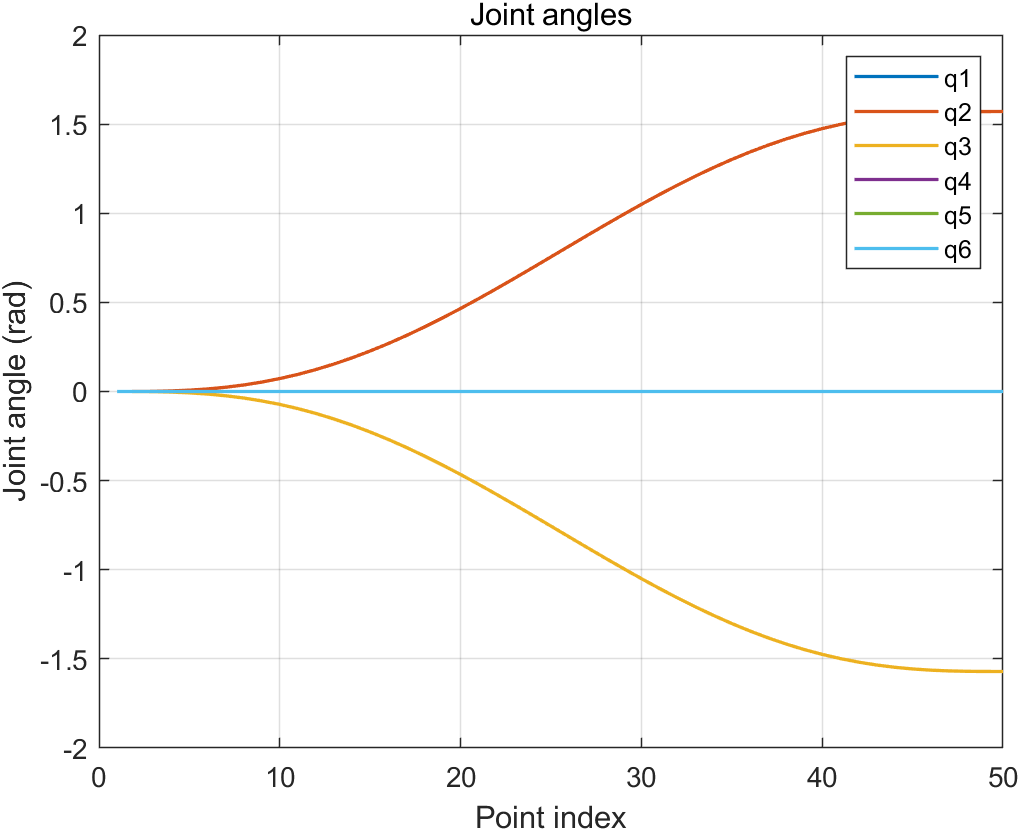
\includegraphics[width=0.78\textwidth]{figures/fig_exp2_joint_angles.png}
  \caption{关节空间规划得到的关节角变化曲线}
  \label{fig:exp2_joint_angles}
\end{figure}

图~\ref{fig:exp2_joint_angles} 为各关节角随采样点的变化情况。可以看到，变化最显著的是第二、第三关节，其中 $q_2$ 从 0 平滑增加至 $\pi/2$，而 $q_3$ 从 0 平滑减小至 $-\pi/2$；其余关节基本保持不变。这与给定的目标关节姿态完全一致，也说明本实验的关节空间规划主要由肩关节和肘关节完成。

\begin{figure}[H]
  \centering
  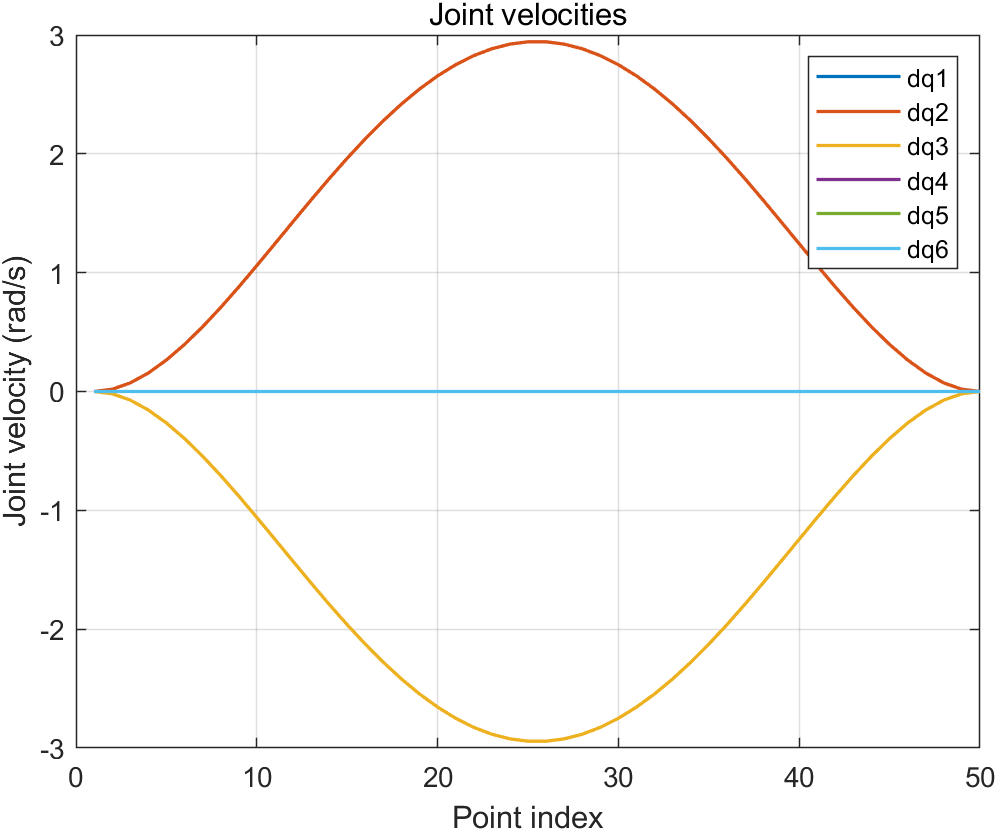
\includegraphics[width=0.78\textwidth]{figures/fig_exp2_joint_velocities.png}
  \caption{关节空间规划得到的关节角速度曲线}
  \label{fig:exp2_joint_velocities}
\end{figure}

图~\ref{fig:exp2_joint_velocities} 展示了关节角速度变化。第二、第三关节的速度曲线关于零轴对称，且在起点和终点均回到零值，符合五次多项式插值边界条件。其速度峰值约为 $\pm 2.9428\,\si{rad/s}$。速度曲线连续光滑，说明 \texttt{jtraj} 在速度层面具有良好的平滑性。

\begin{figure}[H]
  \centering
  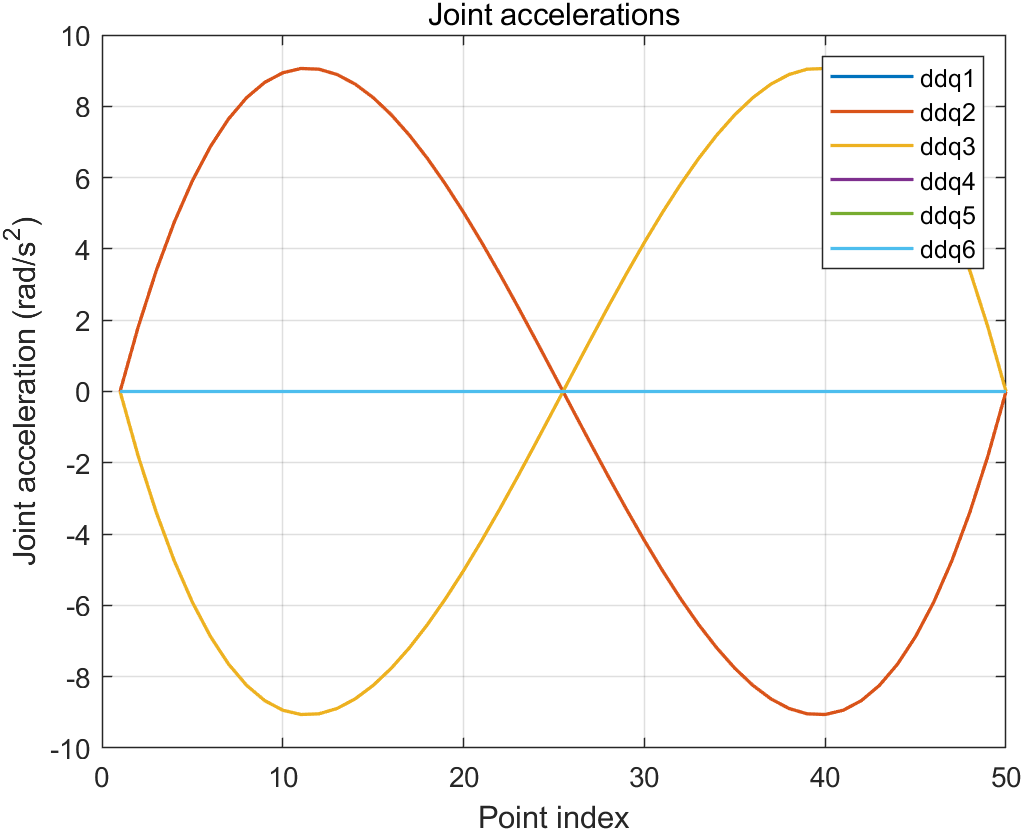
\includegraphics[width=0.78\textwidth]{figures/fig_exp2_joint_accelerations.png}
  \caption{关节空间规划得到的关节角加速度曲线}
  \label{fig:exp2_joint_acc}
\end{figure}

图~\ref{fig:exp2_joint_acc} 给出了关节角加速度曲线。第二、第三关节在起始阶段和结束阶段分别表现出相反方向的加速与减速过程，最大幅值约为 $\pm 9.0604\,\si{rad/s^2}$。曲线在全过程中连续变化，说明插值轨迹满足较好的动态平滑性要求。

\begin{figure}[H]
  \centering
  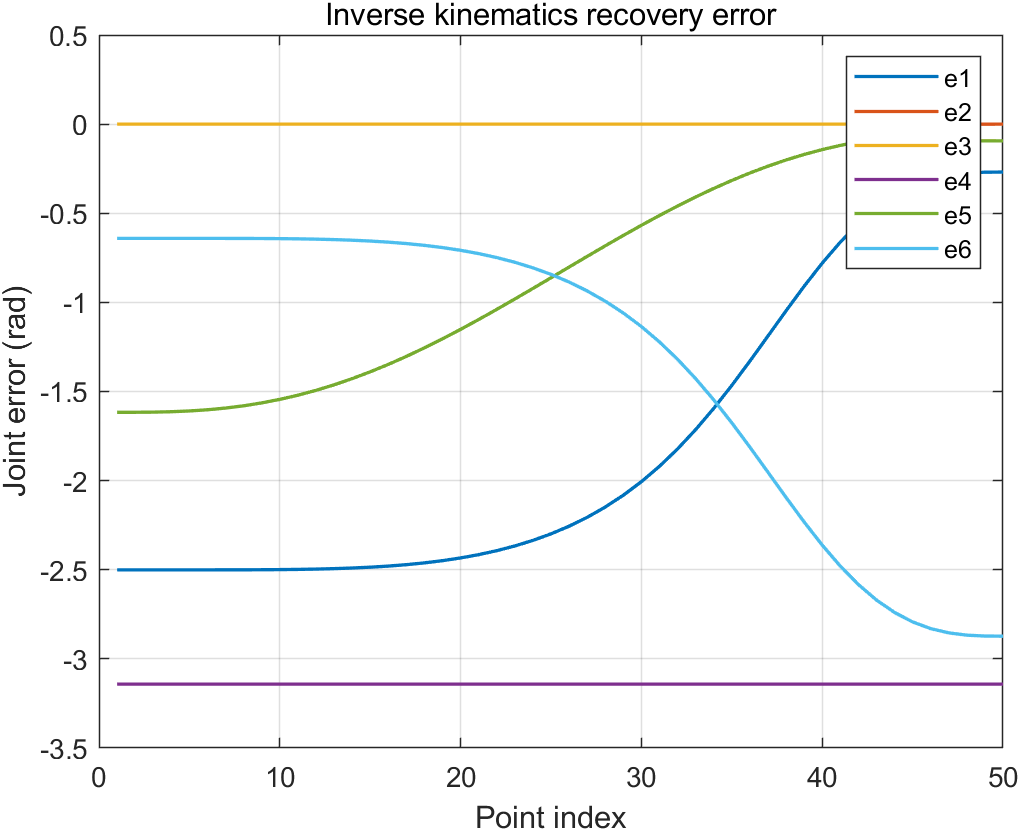
\includegraphics[width=0.78\textwidth]{figures/fig_exp2_ik_error.png}
  \caption{实验二中逆运动学恢复的关节误差曲线}
  \label{fig:exp2_ik_error}
\end{figure}

图~\ref{fig:exp2_ik_error} 反映了将关节空间规划产生的末端位姿再次进行逆运动学求解后，所得关节角与原始关节轨迹之间的差异。从图中可以看出，部分关节误差并未接近零，其中第四关节误差基本保持在 $\pi$ 附近，第一、第二、第五、第六关节也存在较大偏差，而第三关节误差相对较小。各关节最大绝对恢复误差约为
\begin{equation}
\left[2.5007,\ 1.6167,\ 0.0940,\ \pi,\ 1.6167,\ 2.8726\right]\ \si{rad}.
\end{equation}

这一现象说明，逆运动学恢复的是“能够实现同一末端位姿的某一组合法关节解”，而不是必然恢复出原始规划关节轨迹。对六自由度机械臂而言，不同肘部构型、腕部翻转方式都可能对应相同的末端位姿，因此实验二得到的关节恢复误差主要体现了逆运动学多解性，而不意味着末端位姿计算错误。

\subsection{两种轨迹规划方式的对比分析}

结合实验一与实验二结果，可以得到如下认识：
\begin{enumerate}
  \item 笛卡尔空间规划直接约束末端执行器的位姿变化，因此更适合末端路径有明确几何要求的任务，如抓取、焊接和喷涂等。实验一中末端规划轨迹与验证轨迹几乎完全重合，说明该方法在几何路径控制方面具有明确优势。
  \item 关节空间规划直接规划关节变量，因此计算过程简单、轨迹平滑性好，便于满足驱动层面的速度和加速度约束。实验二中关节角、角速度和角加速度曲线均较平滑，体现了该方法的工程实用性。
  \item 关节空间规划下的末端轨迹通常不具备直观的几何可控性，图~\ref{fig:exp2_ee_traj} 中的弯曲轨迹即说明了这一点。
  \item 逆运动学求解存在多解性。实验二中恢复关节角与原始关节轨迹差异较大，但末端位姿依然能够保持一致，这从侧面说明在机器人控制与规划中应根据构型约束、连续性约束和初值条件选择合适的逆解分支。
\end{enumerate}

\section{关键代码展示}

下列代码片段概括了本实验两个部分的核心实现过程：实验一通过“笛卡尔轨迹规划 $\rightarrow$ 逆运动学 $\rightarrow$ 正运动学验证”完成闭环验证；实验二通过“关节轨迹规划 $\rightarrow$ 正运动学 $\rightarrow$ 逆运动学恢复”分析逆解特性。

\begin{lstlisting}[style=matlabstyle,caption={实验关键 MATLAB 代码片段},label={lst:keycode}]
clc; clear; close all;
mdl_puma560

q_start = qz;
q_end   = qr;
n = 50;

% Experiment 1: Cartesian trajectory planning and FK verification
T_start = p560.fkine(q_start);
T_end   = p560.fkine(q_end);
Ts      = ctraj(T_start, T_end, n);
q_traj  = p560.ikine6s(Ts);

for i = 1:n
    xyz_plan(i,:) = transl(Ts(i));
    T_now = p560.fkine(q_traj(i,:));
    xyz_fk(i,:) = transl(T_now);
end
err = sqrt(sum((xyz_plan - xyz_fk).^2, 2));

% Experiment 2: Joint-space planning and IK recovery
[q, qd, qdd] = jtraj(q_start, q_end, n);
for i = 1:n
    Ts2(:,:,i) = p560.fkine(q(i,:));
    q_ik(i,:)  = p560.ikine6s(Ts2(:,:,i));
end
q_err = atan2(sin(q - q_ik), cos(q - q_ik));
\end{lstlisting}

代码~\ref{lst:keycode} 对应了实验报告中的核心分析链条。第一部分先在位姿空间生成末端轨迹，再通过逆解和正解回代计算位置误差；第二部分则在关节空间生成平滑轨迹，并通过逆运动学恢复关节角以评估多解性对结果的影响。

\section{实验结论}

本实验基于 MATLAB Robotics Toolbox 完成了 PUMA560 机械臂的正运动学、逆运动学与轨迹规划仿真。通过对笛卡尔空间和关节空间两种规划方式的对比分析，可以得到以下结论：
\begin{enumerate}
  \item 在笛卡尔空间下进行轨迹规划时，末端执行器的目标轨迹可以通过逆运动学准确映射到关节空间，再经正运动学回代后与原规划轨迹基本完全重合，验证误差仅为数值精度级别。
  \item 在关节空间下进行轨迹规划时，各关节角、角速度和角加速度均具有良好的连续性与平滑性，但其对应的末端空间轨迹通常并非直线，而是由机构几何关系共同决定的空间曲线。
  \item 对关节空间规划得到的末端位姿再次求取逆运动学时，恢复出的关节角与原始关节轨迹不一定一致，说明逆运动学存在多组可行解。因而在实际应用中，逆解不仅要满足末端位姿要求，还应综合考虑构型连续性、避障需求和驱动约束。
  \item 本实验较完整地展示了“由关节求位姿”和“由位姿求关节”两类问题的求解过程，验证了 PUMA560 模型与 MATLAB Robotics Toolbox 的有效性，并加深了对工业机器人运动学分析方法的理解。
\end{enumerate}

\end{document}
